\section{Desarrollo/Análisis}
Gracias a lo consultado en \cite{web3}, fue posible realizar todas las configuraciones necesarias para empezar con el uso del programa \texttt{IMU\_ Capture.ino} disponible en \cite{ArduinoSketches1}, el cual se encarga de leer la aceleración y el giroscopio de la placa e imprime por un segundo en el monitor serial (por consola del IDE) cuando una velocidad significativa es detectada. Además, es posible activar el \texttt{Serial Plotter} para graficar los datos. Lo anterior se muestra a continuación.

\begin{figure}[H]
   \begin{minipage}{0.48\textwidth}
     \centering
     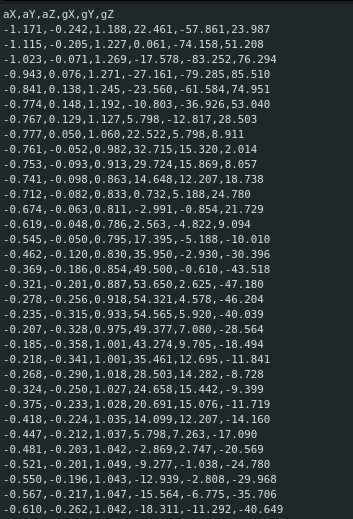
\includegraphics[width=.7\linewidth]{Imagenes/4}
     \caption{ Registro del giroscopio}\label{Fig_4}
   \end{minipage}\hfill
   \begin{minipage}{0.7\textwidth}
     \centering
     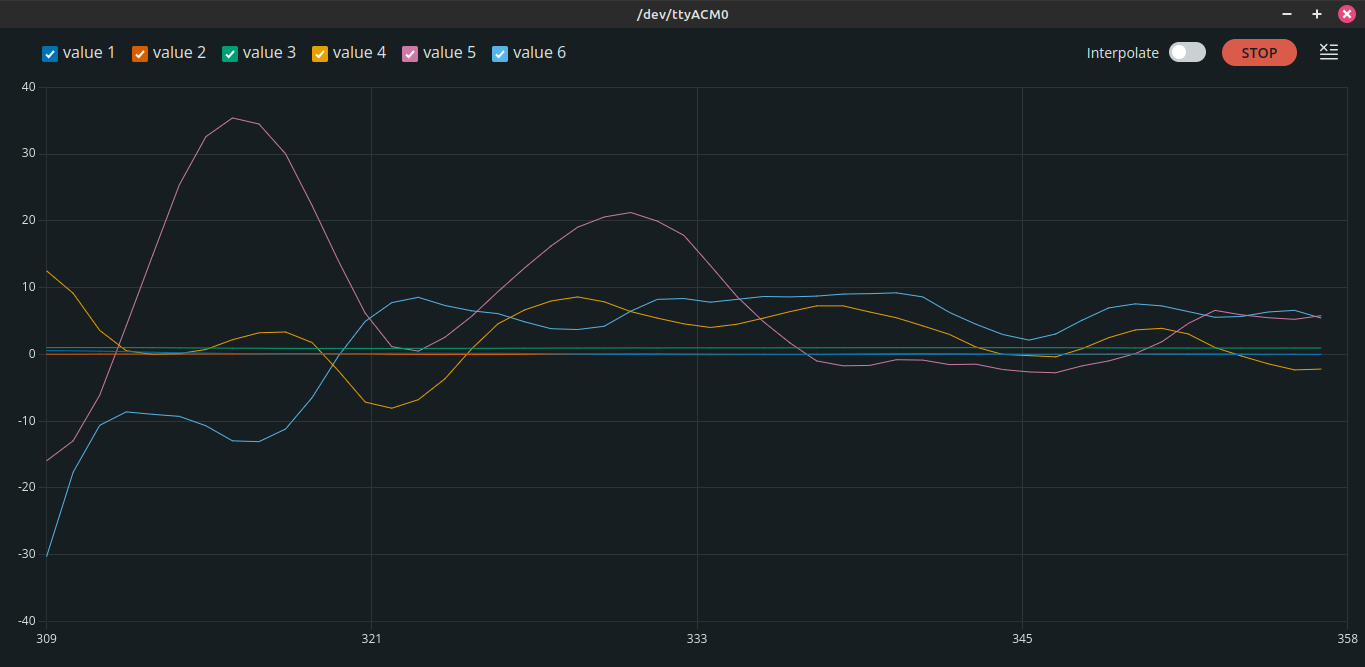
\includegraphics[width=.7\linewidth]{Imagenes/5.png}
     \caption{Graficación del movimiento }\label{Fig_5}
   \end{minipage}
\end{figure}
De la figura \ref{Fig_4}, se tiene las coordenadas que registran el movimiento realizado, que de hecho es un golpe hacia la pantalla de la PC. Luego, en la figura \ref{Fig_5} muestra las ondas del golpe. Hecho esto, se procede a realizar un pequeño script de Python para grabar todos estos datos en un archivo .csv. Por lo que una vez cargado el código \texttt{IMU\_ Capture.ino} se cierra el IDE de Arduino y se ejecuta el script. De donde se realizaron 3 movimientos.
\begin{itemize}
\item Golpe hacia la pantalla (en una sola dirección).
\item Alzar el brazo con diferentes direcciones.
 \item Movimiento circular en contra de las manecillas del reloj.
\end{itemize}
Se tomaron 1750 muestras para los 3 movimientos, un aproximado de \SI{25}{\s} realizando la misma tarea. Ahora, con base a estos datos se realizó el entrenamiento con ayuda de \cite{web4}.\par

%\begin{figure}[H]
%\centering
%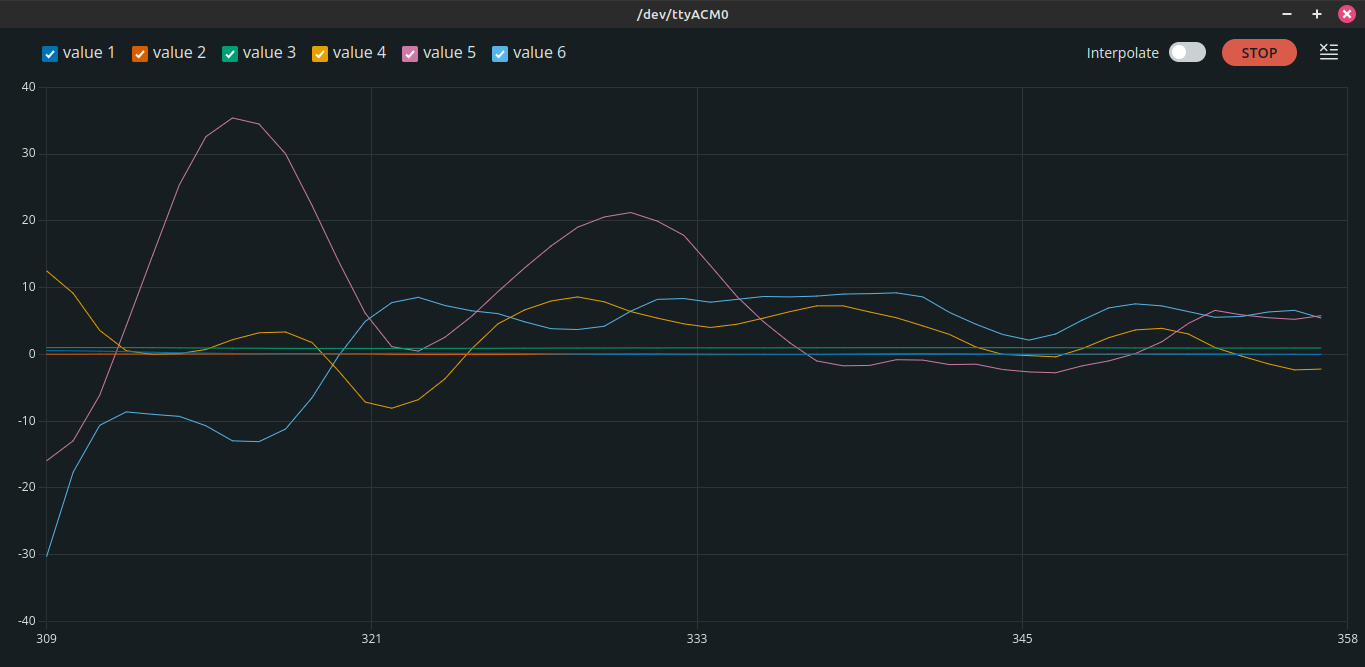
\includegraphics[width=.55\linewidth]{Imagenes/5.png}
% \caption{Funcionamiento del giroscopio.}
% \label{fig_gyro}
%\end{figure}

Para el entrenamiento se tomaron los resultados obtenidos y se procedió a usar como base el ejemplo de reconocimiento de gestos dado en la presentación de la clase \cite{web4}.
El primer paso fue introducir los datos, el resultado de esto se observa a continuación:
\begin{figure}[H]
    \centering
    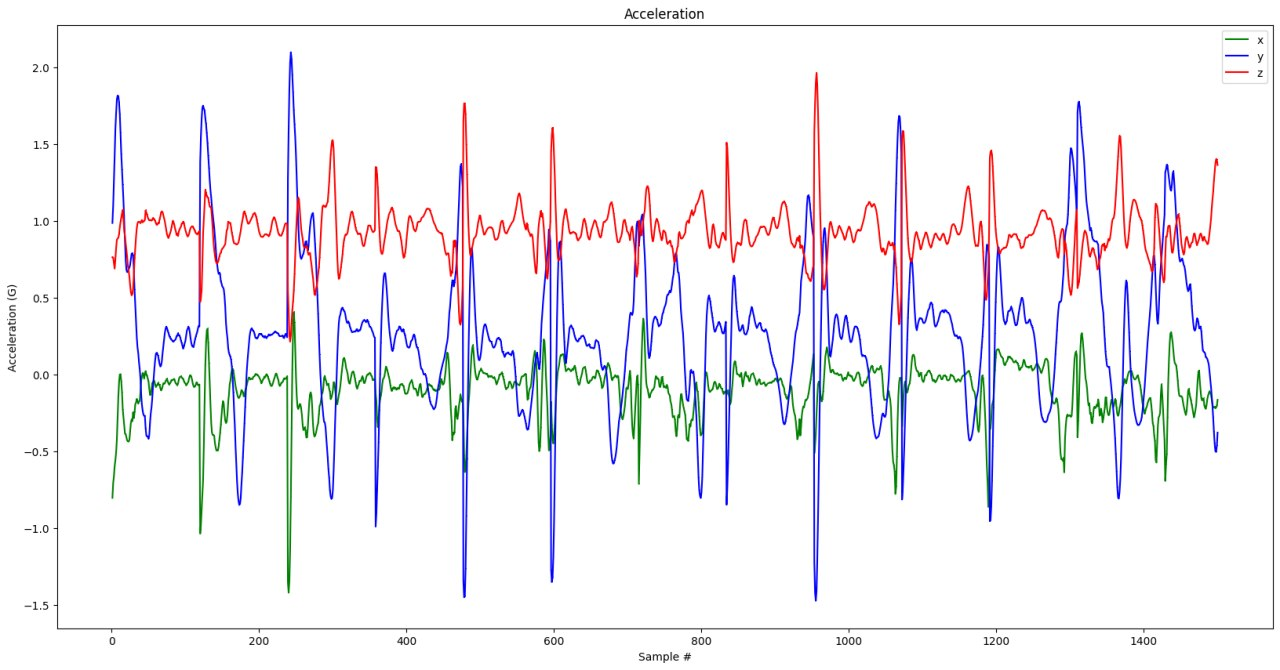
\includegraphics[width=.65\linewidth]{Imagenes/k (1).jpg}
    \caption{Datos de aceleración importados.}
\end{figure}

\begin{figure}[H]
    \centering
    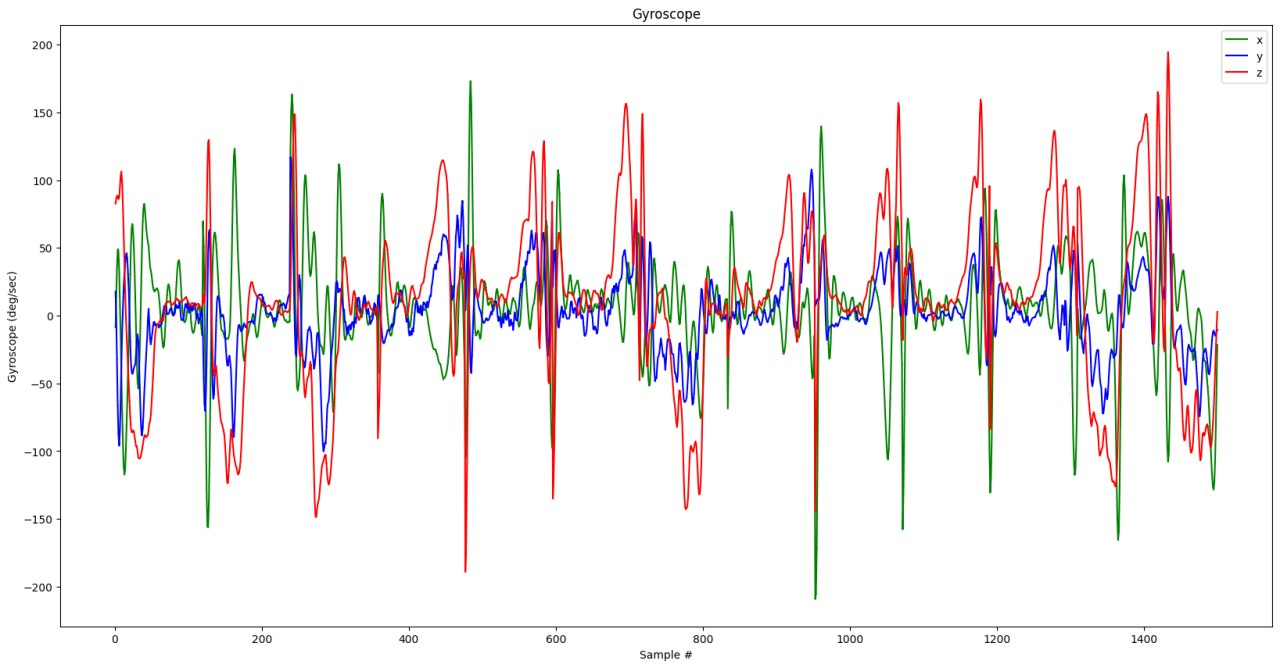
\includegraphics[width=.65\linewidth]{Imagenes/k (2).jpg}
    \caption{Datos del giroscopio importado.}
\end{figure}

Una vez realizado este paso se empieza a entrenar el modelo, para ello se preparan los datos para que su formato coincida, una vez realizado lo anterior se entrena la red siguiendo las indicaciones del enunciado y tomando el 60\% de los datos para el entrenamiento, un 20\% para la validación y otro 20\% para realizar pruebas. Los resultados del entrenamiento se muestran en las siguientes figuras:
\begin{figure}[H]
    \centering
    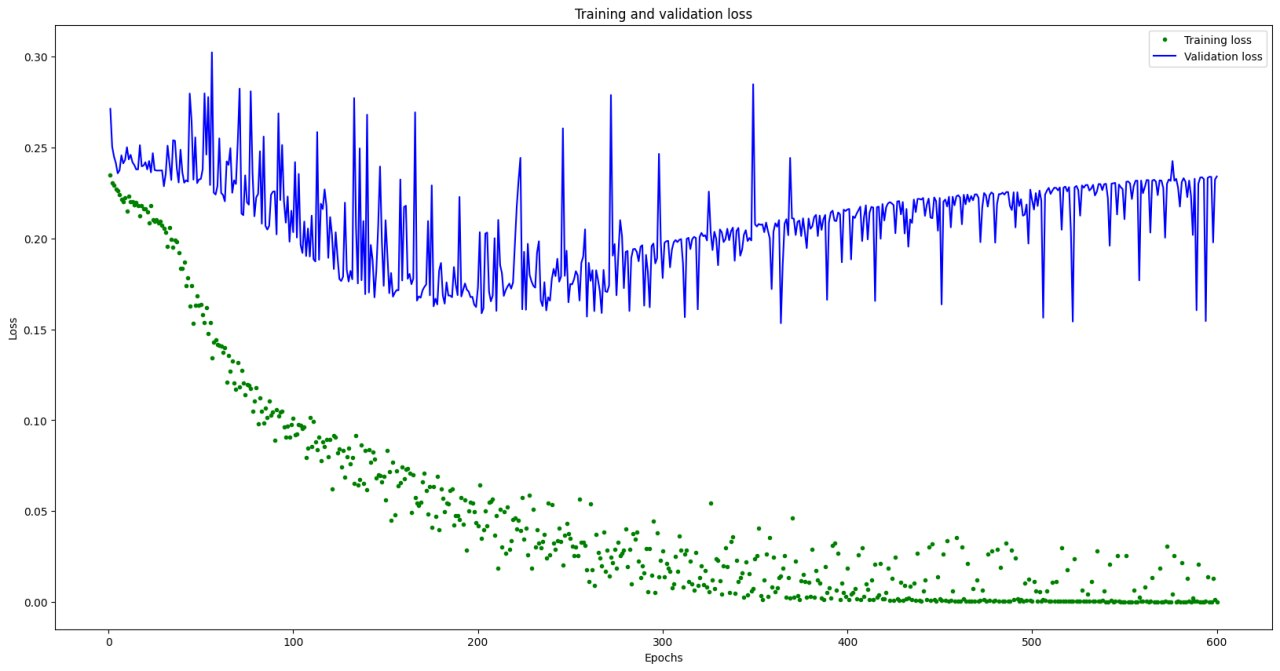
\includegraphics[width=.65\linewidth]{Imagenes/k (3).jpg}
    \caption{Gráfica del entrenamiento y su pérdida.}
\end{figure}

\begin{figure}[H]
    \centering
    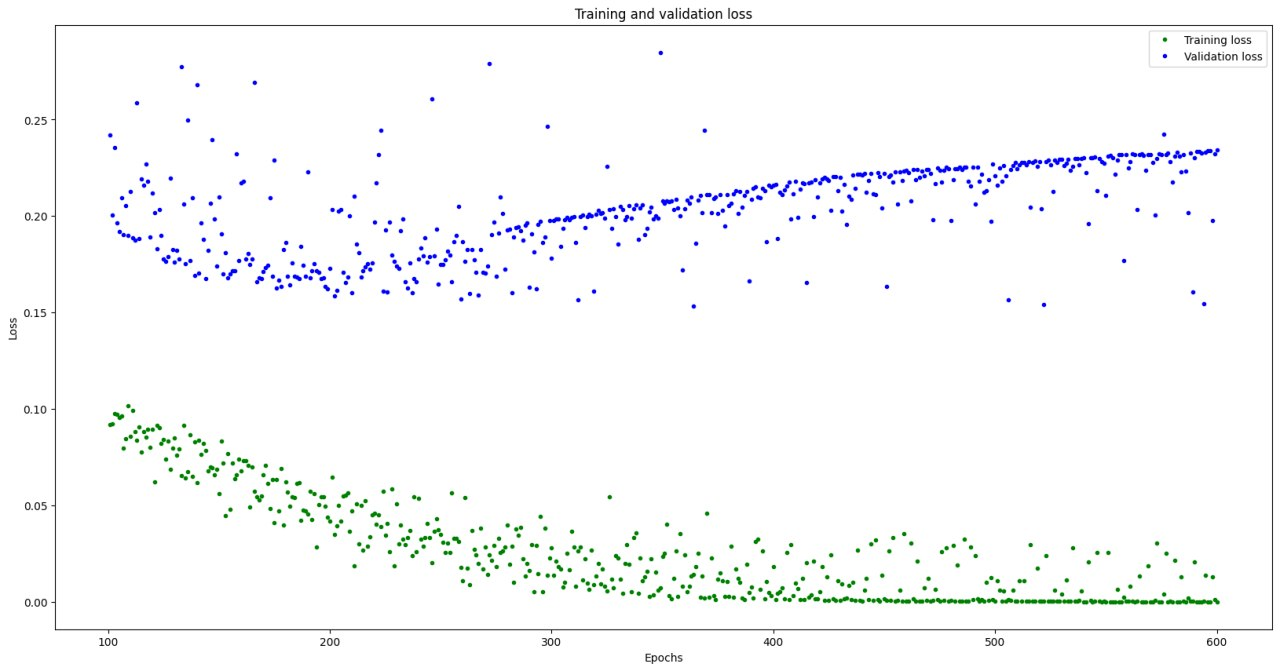
\includegraphics[width=.65\linewidth]{Imagenes/k (4).jpg}
    \caption{Gráfica del entrenamiento y su pérdida iniciando en 100.}
\end{figure}

\begin{figure}[H]
    \centering
    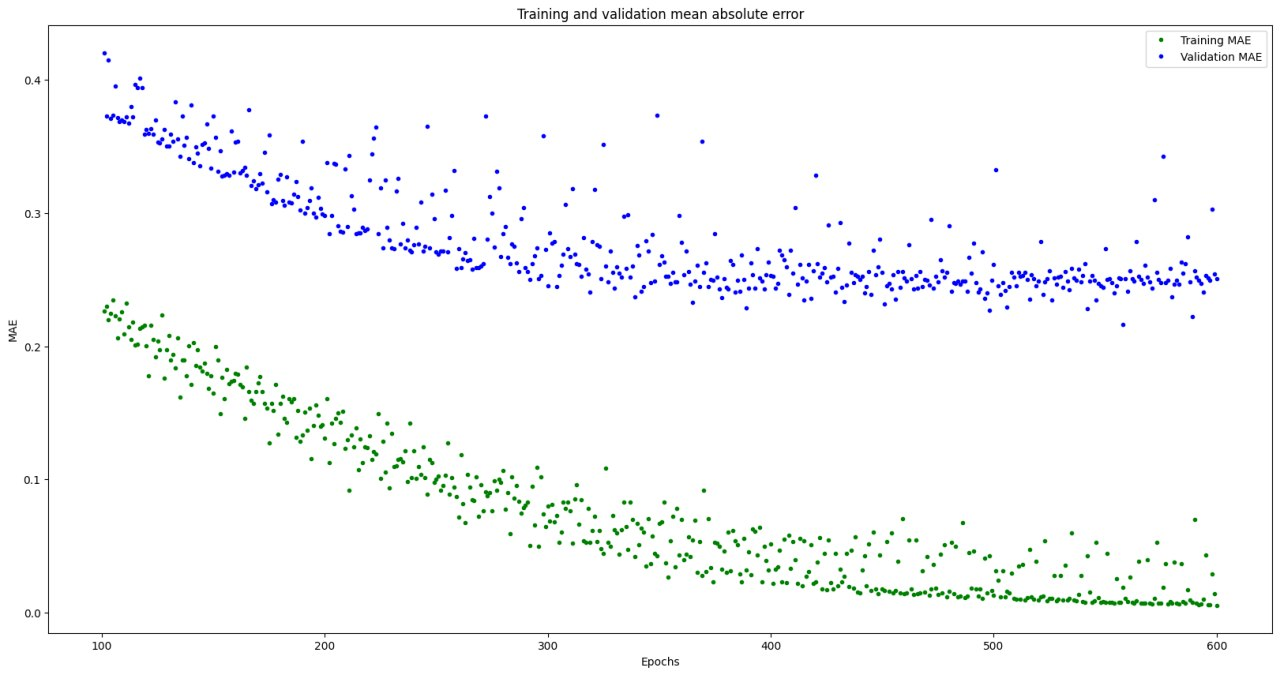
\includegraphics[width=.65\linewidth]{Imagenes/k (5).jpg}
    \caption{Gráfica del error absoluto para observar rendimiento.}
\end{figure}

Con lo anterior se obtiene un archivo de encabezado ''model.h'' que es usado para poder determinar los movimientos escogidos para este laboratorio.\\

Ahora, gracias al entrenamiento realizado y siguiendo con la ayuda de los ejemplos vistos en clase, se toma la referencia de \cite{ArduinoSketches1} a la cual se le hacen unas pequeñas modificaciones, primero se le añade el archivo \texttt{model.h} para ver los resultados del entramiento pero ahora en la placa.
Lo otro es la eliminación de algunos encabezados que no serán necesarios ya que el profesor indicó que son más orientados a los desarrolladores de tensorflow tales como: \texttt{tensorflow/lite/micro/micro\_error\_ reporter.h} y \texttt{tensorflow/lite/version.h}. También se eliminó la variable global \texttt{tflite::MicroErrorReporter tflErrorReporter} y el acceso a la memoria de esta misma variable. Por otro, lado se tuvo que añadir los mapas de los gestos:\newpage
\begin{lstlisting}[label={mini_bloque}, caption={Nombre de los archivos csv}]
// array to map gesture index to a name
const char* GESTURES[] = {
  "punch",
  "arm_up",
  "circle"
};
\end{lstlisting}

Hecho esto, se verificó y cargó el código a la placa, lo cual tomó cierto tiempo en comparación a otros ejemplos. Una vez terminado esto, se realizaron los movimientos y por medio del serial monitor se mostraron las probabilidades de los movimientos ejecutados, donde el que posee mayor probabilidad indica  el movimiento o acción hecha con la placa.
\begin{figure}[H]
   \begin{minipage}{0.5\textwidth}
     \centering
     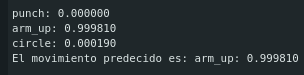
\includegraphics[width=.48\linewidth]{Imagenes/arm_up.png}
     \caption{ Movimiento brazo arriba.}\label{arm_up}
   \end{minipage}\hfill
   \begin{minipage}{0.5\textwidth}
     \centering
     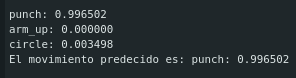
\includegraphics[width=.48\linewidth]{Imagenes/punch.png}
     \caption{Movimiento puño hacia la PC. }\label{punch}
   \end{minipage}
      \begin{minipage}{0.5\textwidth}
     \centering
     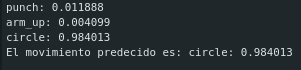
\includegraphics[width=.48\linewidth]{Imagenes/circle.png}
     \caption{Movimiento circular. }\label{circle}
   \end{minipage}
    \begin{minipage}{0.5\textwidth}
     \centering
     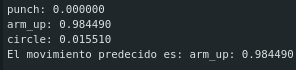
\includegraphics[width=.48\linewidth]{Imagenes/brazo_up.png}
     \caption{Movimiento brazo arriba. }\label{brazo_up}
   \end{minipage}
\end{figure}
Primero se levantó el brazo y es sencillo notar que en la figura \ref{arm_up} el movimiento es detectado correctamente ya que las demás probabilidades o valores con base al entrenamiento fueron totalmente despreciables. El siguiente movimiento fue un puñetazo hacia la PC y note que en la figura \ref{punch} la placa logra detectarlo sin problema alguno, con una similitud muy ínfima con el movimiento circular. Por último, se movió la placa en forma circular y el resultado de la figura \ref{circle} detecta este movimiento con algunas similitudes con el levantamiento del brazo hacia y el puñetazo, no obstante el valor más alto fue el movimiento circular. En resumen, la figura \ref{moves} es la consola o el monitor serial de Arduino que va mostrando estas probabilidades dependiendo del movimiento que se ejecute con la placa.
\begin{figure}[H]
\centering
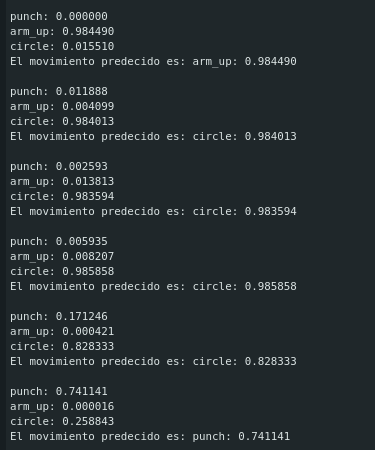
\includegraphics[width=.40\linewidth]{Imagenes/11.png}
 \caption{Resumen de los movimientos.}
 \label{moves}
\end{figure}

\newpage


\newpage